\chapter{Manual de Utilização da Aplicação Móvel}

O \textbf{ScriptumAI} é uma aplicação móvel para Android que permite gerir documentos organizacionais em qualquer lugar, sem necessidade de aceder à plataforma \textit{web}. Através da aplicação, o utilizador pode carregar documentos, consultar análises geradas por inteligência artificial e interagir com o conteúdo documental através de um assistente conversacional. Este guia descreve como utilizar cada funcionalidade disponível.

\newcommand{\screenshot}[1]{%
    \fbox{\begin{minipage}[c][7cm][c]{\textwidth}
        \centering\small\textit{#1}
    \end{minipage}}%
}

\clearpage
\section{Ecrã de Apresentação e Início de Sessão}

Ao abrir a aplicação é apresentado o ecrã de \textit{splash} com o logótipo do \textbf{ScriptumAI}. Caso não exista sessão ativa, o utilizador é direcionado para o ecrã de \textit{login}, visível no ecrã da direita da Figura~\ref{fig:manual-login}. Para entrar na aplicação, o utilizador preenche o \textit{email} e a palavra-passe e toca no botão ``Entrar''. Caso não tenha conta, pode tocar em ``Registar'' para criar uma.

\begin{figure}[H]
    \centering
    \begin{subfigure}[b]{0.28\textwidth}
        \centering
        \fbox{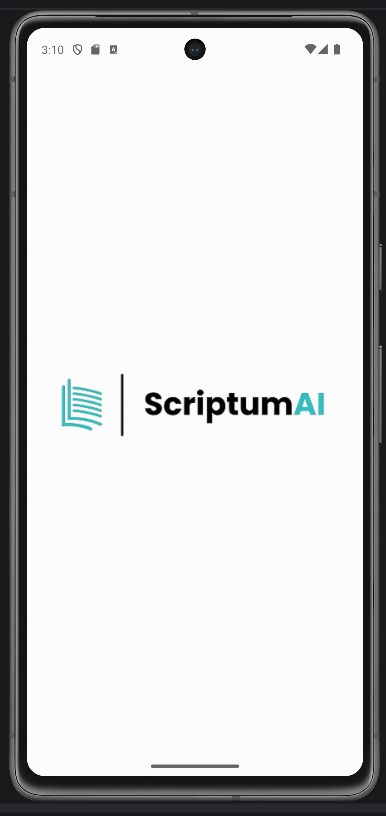
\includegraphics[width=\textwidth]{images/screenshots/splash_screen.png}}
        \caption{\textit{Splash Screen}}
    \end{subfigure}
    \hspace{0.03\textwidth}
    \begin{subfigure}[b]{0.28\textwidth}
        \centering
        \fbox{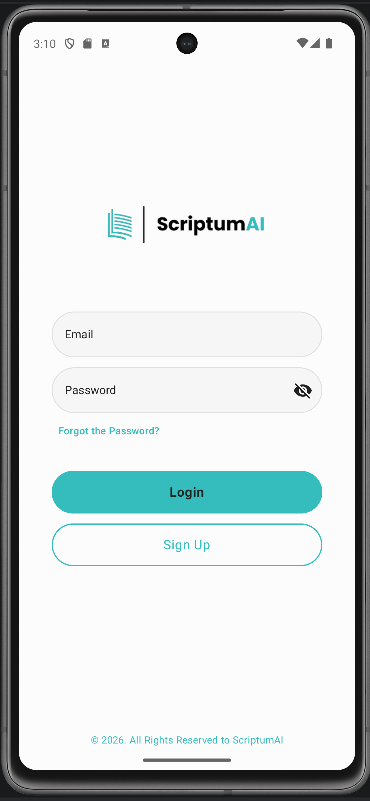
\includegraphics[width=\textwidth]{images/screenshots/login_screen.png}}
        \caption{Início de Sessão}
    \end{subfigure}
    \caption{Ecrã de apresentação e início de sessão.}
    \label{fig:manual-login}
\end{figure}

\clearpage
\section{Recuperação de Palavra-Passe}

Ao tocar em ``Esqueceu a palavra-passe?'' no ecrã de \textit{login}, o utilizador é direcionado para o ecrã da esquerda da Figura~\ref{fig:manual-forgot}, onde introduz o \textit{email} da conta e toca em ``Enviar''. A aplicação envia um \textit{email} com as instruções para redefinir a palavra-passe, sendo depois apresentada a confirmação no ecrã da direita.

\begin{figure}[H]
    \centering
    \begin{subfigure}[b]{0.28\textwidth}
        \centering
        \fbox{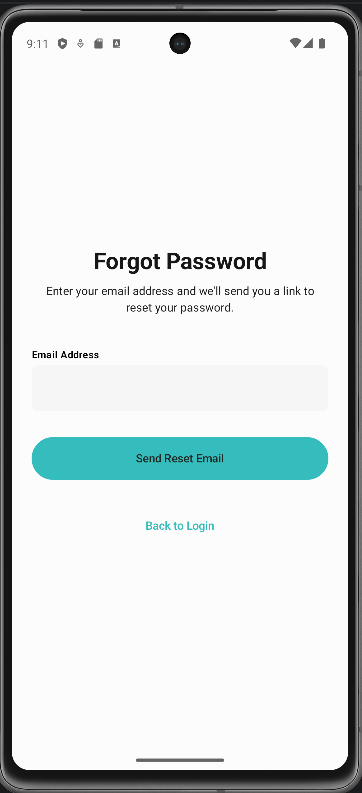
\includegraphics[width=\textwidth]{images/screenshots/forgot_screen.png}}
        \caption{Pedido de Recuperação}
    \end{subfigure}
    \hspace{0.03\textwidth}
    \begin{subfigure}[b]{0.28\textwidth}
        \centering
        \fbox{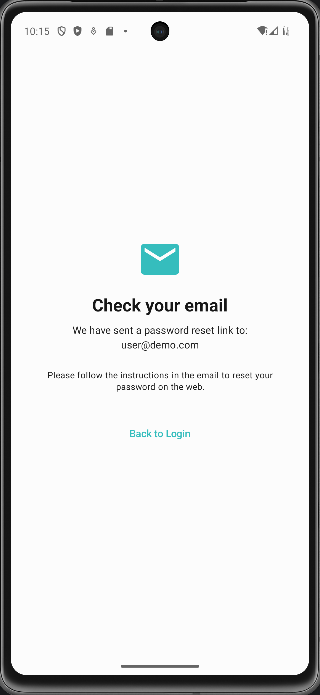
\includegraphics[width=\textwidth]{images/screenshots/confirm_sending_email_screen.png}}
        \caption{Confirmação de Envio}
    \end{subfigure}
    \caption{Recuperação de palavra-passe.}
    \label{fig:manual-forgot}
\end{figure}

\clearpage
\section{Escolha de Plano e Registo}

Antes de criar uma conta, o utilizador escolhe um dos planos de subscrição disponíveis, apresentados no ecrã da esquerda da Figura~\ref{fig:manual-register} e descritos na Tabela~\ref{tab:planos}. Após selecionar o plano, o utilizador preenche o formulário de registo com os dados pessoais e da organização, aceita os Termos e Condições e toca em ``Criar conta e iniciar avaliação''.

\begin{table}[H]
\centering
\small
\begin{tabular}{|l|l|l|l|}
\hline
\textbf{Plano} & \textbf{Preço} & \textbf{Utilizadores} & \textbf{Armazenamento} \\
\hline
Avaliação Gratuita & €0 (15 dias) & - & 500 GB \\
\hline
Starter & €49/mês & Até 10 & 1 TB \\
\hline
Business & €99/mês & Até 30 & 3 TB \\
\hline
Enterprise & Personalizado & Ilimitado & Ilimitado \\
\hline
\end{tabular}
\caption{Planos de subscrição disponíveis no ScriptumAI.}
\label{tab:planos}
\end{table}

\begin{figure}[H]
    \centering
    \begin{subfigure}[b]{0.28\textwidth}
        \centering
        \fbox{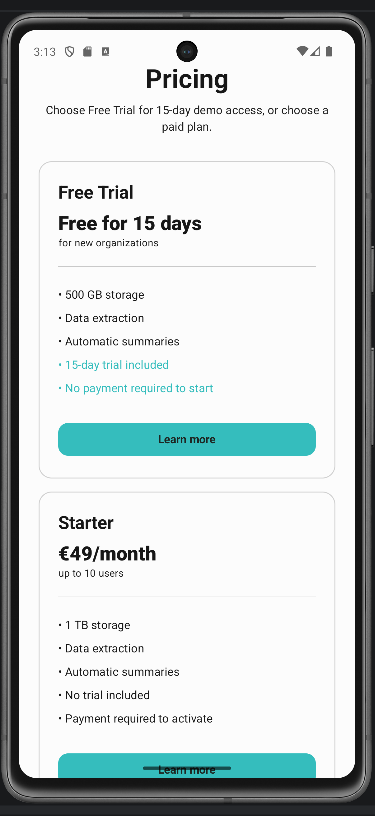
\includegraphics[width=\textwidth]{images/screenshots/plans_screen.png}}
        \caption{Lista de Planos}
    \end{subfigure}
    \hspace{0.03\textwidth}
    \begin{subfigure}[b]{0.28\textwidth}
        \centering
        \fbox{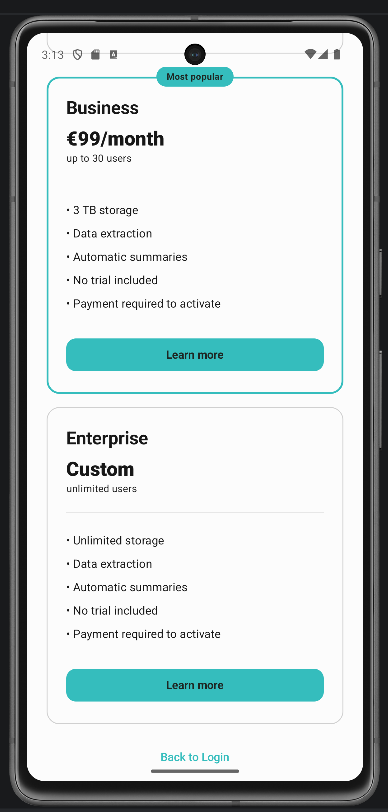
\includegraphics[width=\textwidth]{images/screenshots/plans_screen2.png}}
        \caption{Detalhe do Plano}
    \end{subfigure}
    \caption{Ecrãs de seleção de plano.}
    \label{fig:manual-plans}
\end{figure}

Ao tocar em ``Learn More'' num plano, o utilizador é direcionado para o ecrã de registo, onde preenche os dados pessoais e da organização, como mostra a Figura~\ref{fig:manual-register}. Após aceitar os Termos e Condições, toca em ``Criar conta e iniciar avaliação'' para concluir o registo.

\begin{figure}[H]
    \centering
    \begin{subfigure}[b]{0.28\textwidth}
        \centering
        \fbox{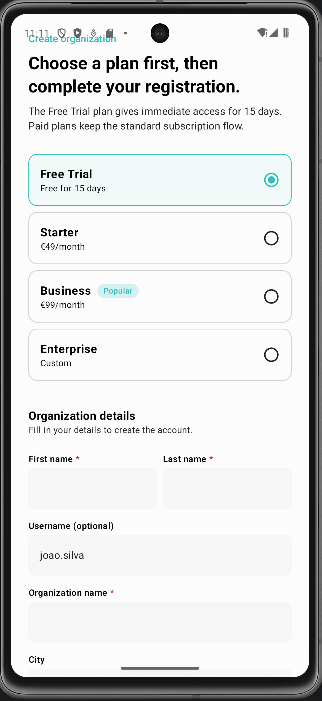
\includegraphics[width=\textwidth]{images/screenshots/choose_plan_screen.png}}
        \caption{Formulário de Registo}
    \end{subfigure}
    \hspace{0.03\textwidth}
    \begin{subfigure}[b]{0.28\textwidth}
        \centering
        \fbox{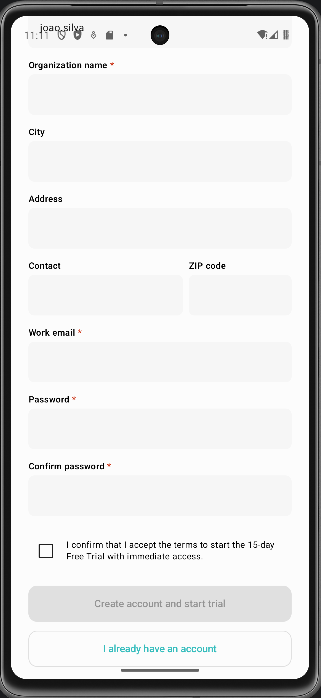
\includegraphics[width=\textwidth]{images/screenshots/choose_plan_screen_2.png}}
        \caption{Confirmação de Dados}
    \end{subfigure}
    \caption{Formulário de registo após seleção do plano.}
    \label{fig:manual-register}
\end{figure}

\clearpage
\section{Dashboard}

Após o início de sessão, o utilizador é direcionado para o \textit{Dashboard}, apresentado na Figura~\ref{fig:manual-dashboard}. Neste ecrã pode ver uma mensagem de boas-vindas, as estatísticas dos documentos da organização (total carregados, processados e pendentes) e uma lista com os 5 documentos mais recentes. Ao tocar num documento, o utilizador é direcionado para o respetivo ecrã de detalhe.

\begin{figure}[H]
    \centering
    \begin{subfigure}[b]{0.28\textwidth}
        \centering
        \fbox{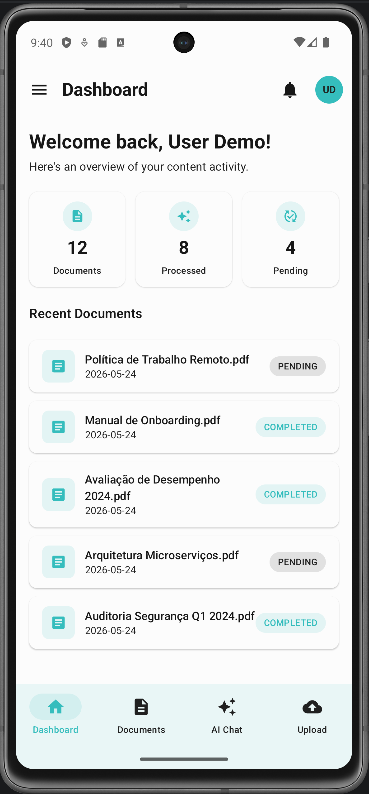
\includegraphics[width=\textwidth]{images/screenshots/dashboard_screen.png}}
        \caption{\textit{Dashboard}}
    \end{subfigure}
    \caption{\textit{Dashboard} com estatísticas e documentos recentes.}
    \label{fig:manual-dashboard}
\end{figure}

\clearpage
\section{Lista de Documentos}

Ao aceder ao separador ``Documentos'', o utilizador vê a lista de todos os documentos da organização, como mostra o ecrã da esquerda da Figura~\ref{fig:manual-documents}. Para encontrar um documento específico, pode usar a barra de pesquisa no topo, filtrar por departamento ou ordenar por data, nome ou tamanho, tocando no ícone de ordenação, como mostra o ecrã da direita.

\begin{figure}[H]
    \centering
    \begin{subfigure}[b]{0.28\textwidth}
        \centering
        \fbox{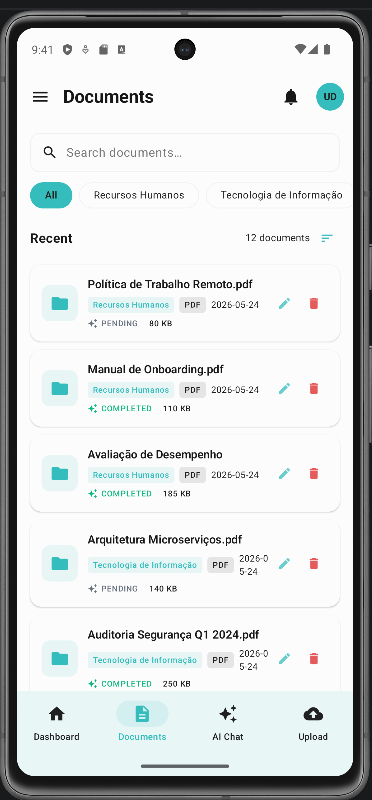
\includegraphics[width=\textwidth]{images/screenshots/documents_screen.png}}
        \caption{Lista de Documentos}
    \end{subfigure}
    \hspace{0.03\textwidth}
    \begin{subfigure}[b]{0.28\textwidth}
        \centering
        \fbox{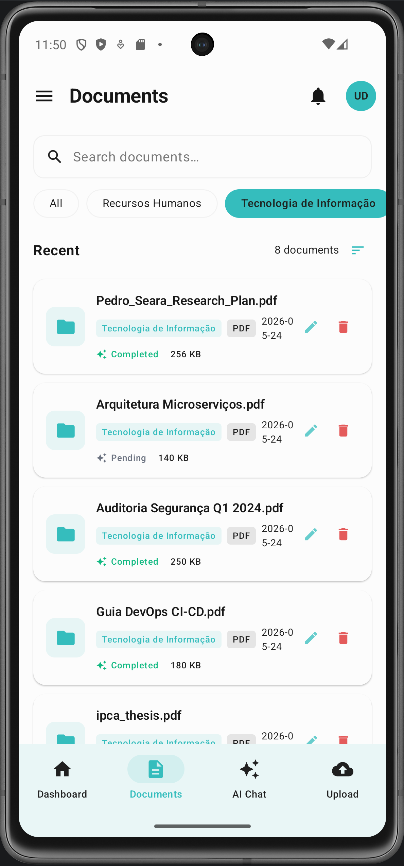
\includegraphics[width=\textwidth]{images/screenshots/search_filters.png}}
        \caption{Pesquisa e Filtros}
    \end{subfigure}
    \caption{Lista de documentos com pesquisa, filtros e ordenação.}
    \label{fig:manual-documents}
\end{figure}

\clearpage
\section{Detalhe do Documento e Análise IA}

Ao tocar num documento da lista, o utilizador é direcionado para o ecrã de detalhe, visível no ecrã da esquerda da Figura~\ref{fig:manual-detail}, onde pode ver todos os metadados do documento. Após o processamento pela IA, é apresentada a secção de análise no ecrã da direita, com o resumo automático, palavras-chave, entidades identificadas e a pontuação de confiança da análise. Neste ecrã estão também disponíveis as ações de descarregar, partilhar, editar e eliminar o documento.

\begin{figure}[H]
    \centering
    \begin{subfigure}[b]{0.28\textwidth}
        \centering
        \fbox{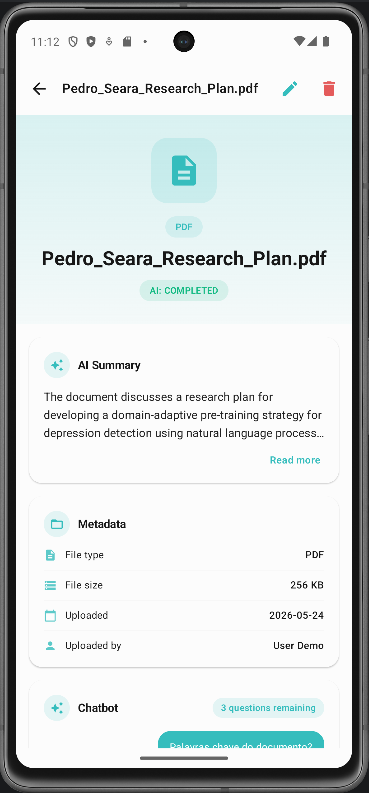
\includegraphics[width=\textwidth]{images/screenshots/metadata.png}}
        \caption{Metadados}
    \end{subfigure}
    \hspace{0.03\textwidth}
    \begin{subfigure}[b]{0.28\textwidth}
        \centering
        \fbox{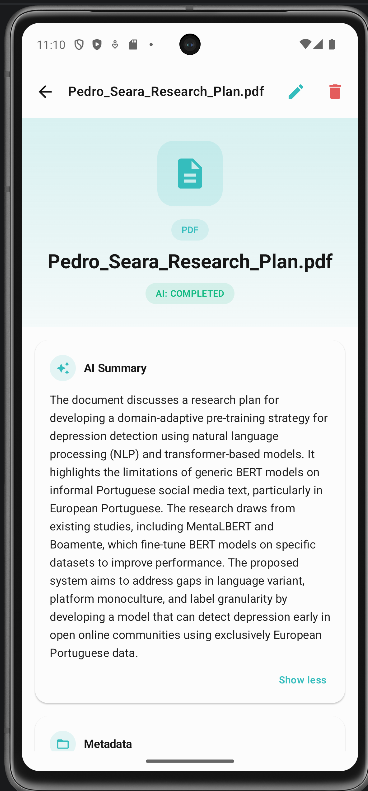
\includegraphics[width=\textwidth]{images/screenshots/ai_analyse.png}}
        \caption{Análise IA}
    \end{subfigure}
    \caption{Ecrã de detalhe do documento e análise por IA.}
    \label{fig:manual-detail}
\end{figure}

\clearpage
\section{Chat por Documento}

No ecrã de detalhe de um documento, o utilizador pode fazer perguntas diretamente sobre o seu conteúdo através da secção de \textit{chat}, apresentada no ecrã da esquerda da Figura~\ref{fig:manual-doc-chat}. O utilizador escreve a pergunta e toca no botão de envio; a IA responde com base no conteúdo do documento. Quando a quota de perguntas é esgotada, o campo de texto fica desativado e é apresentada uma mensagem de aviso, como mostra o ecrã da direita.

\begin{figure}[H]
    \centering
    \begin{subfigure}[b]{0.28\textwidth}
        \centering
        \fbox{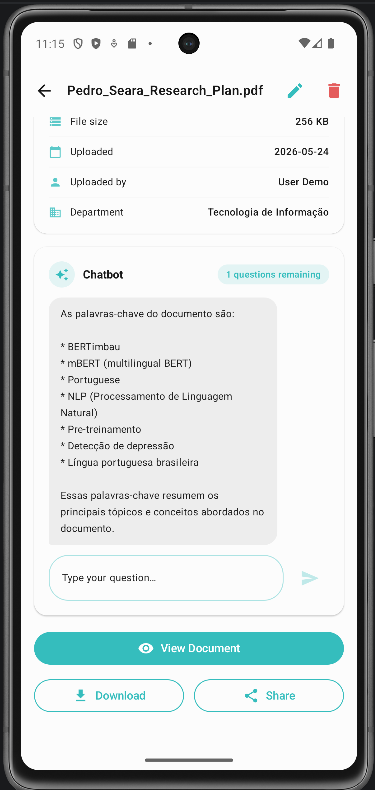
\includegraphics[width=\textwidth]{images/screenshots/active_chatbot_document.png}}
        \caption{\textit{Chat} Ativo}
    \end{subfigure}
    \hspace{0.03\textwidth}
    \begin{subfigure}[b]{0.28\textwidth}
        \centering
        \fbox{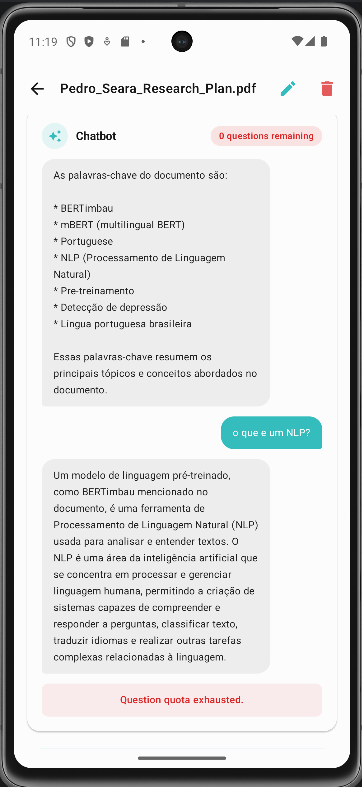
\includegraphics[width=\textwidth]{images/screenshots/quota_exhausted.png}}
        \caption{Quota Esgotada}
    \end{subfigure}
    \caption{\textit{Chat} por documento com sistema de quotas.}
    \label{fig:manual-doc-chat}
\end{figure}

\clearpage
\section{Adicionar Documento}

No separador ``Adicionar'', o utilizador tem duas formas de carregar um documento. Ao tocar em ``\textit{Upload}'', abre o seletor de ficheiros do dispositivo, onde seleciona o ficheiro pretendido. Ao tocar em ``Digitalizar Documento'', abre a câmara em modo de deteção automática de documentos com tecnologia \textit{ML Kit}, que corrige a perspetiva e converte a captura para PDF. Em ambos os casos, o utilizador preenche o nome, uma descrição opcional e seleciona o departamento antes de tocar em ``Guardar'', como mostram os ecrãs da Figura~\ref{fig:manual-upload}.

\begin{figure}[H]
    \centering
    \begin{subfigure}[b]{0.28\textwidth}
        \centering
        \fbox{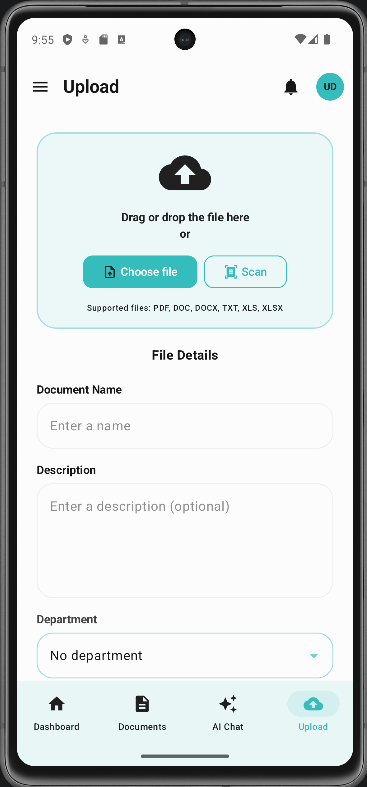
\includegraphics[width=\textwidth]{images/screenshots/upload_doc_screen.png}}
        \caption{Formulário de \textit{Upload}}
    \end{subfigure}
    \hspace{0.03\textwidth}
    \begin{subfigure}[b]{0.28\textwidth}
        \centering
        \fbox{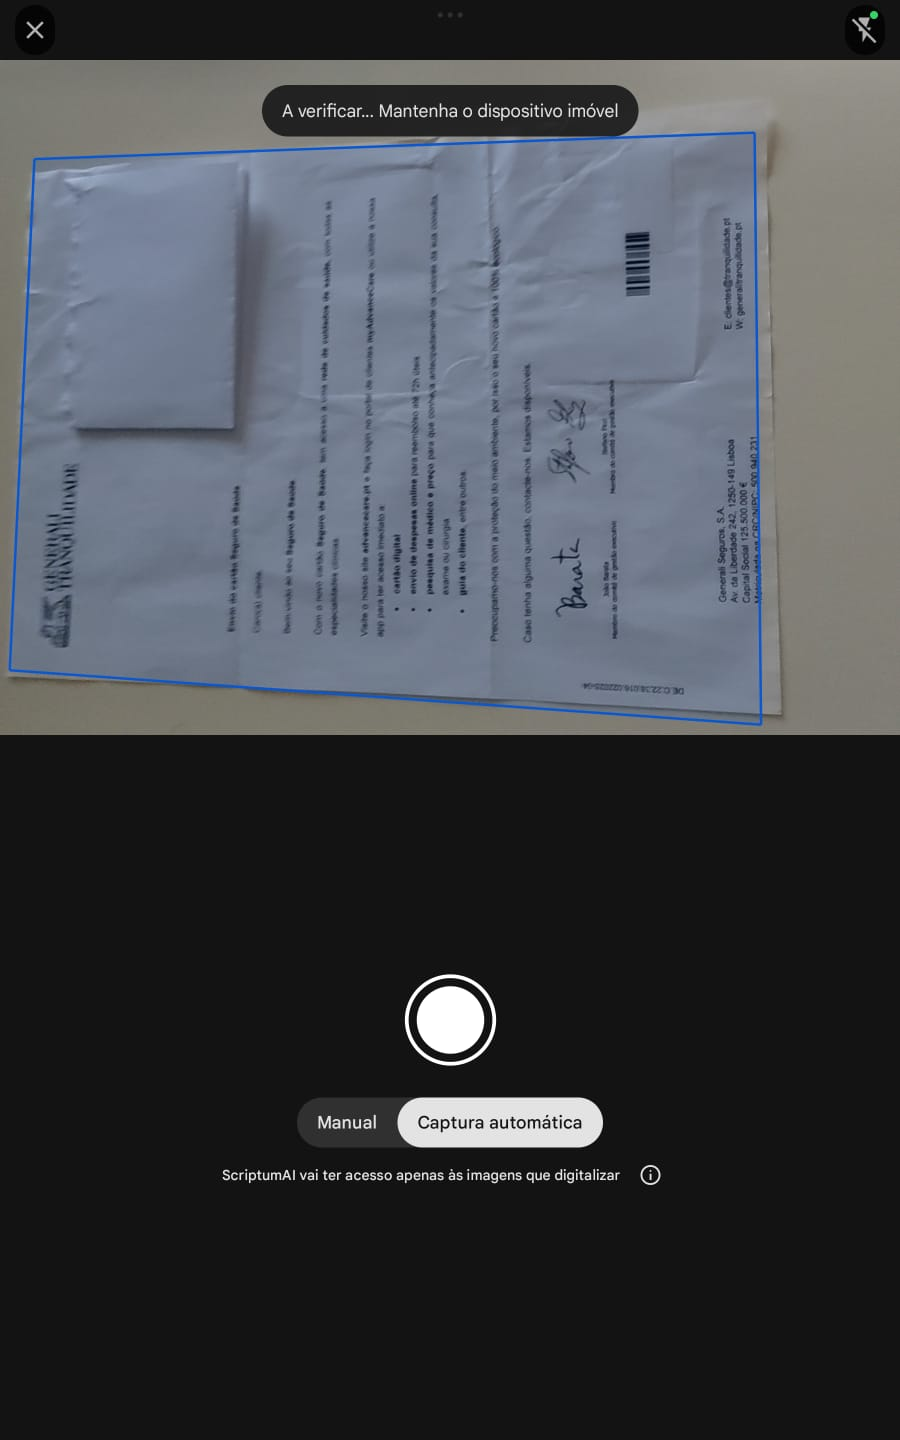
\includegraphics[width=\textwidth]{images/screenshots/scan_screen.jpeg}}
        \caption{Digitalizador com Câmara}
    \end{subfigure}
    \hspace{0.03\textwidth}
    \begin{subfigure}[b]{0.28\textwidth}
        \centering
        \fbox{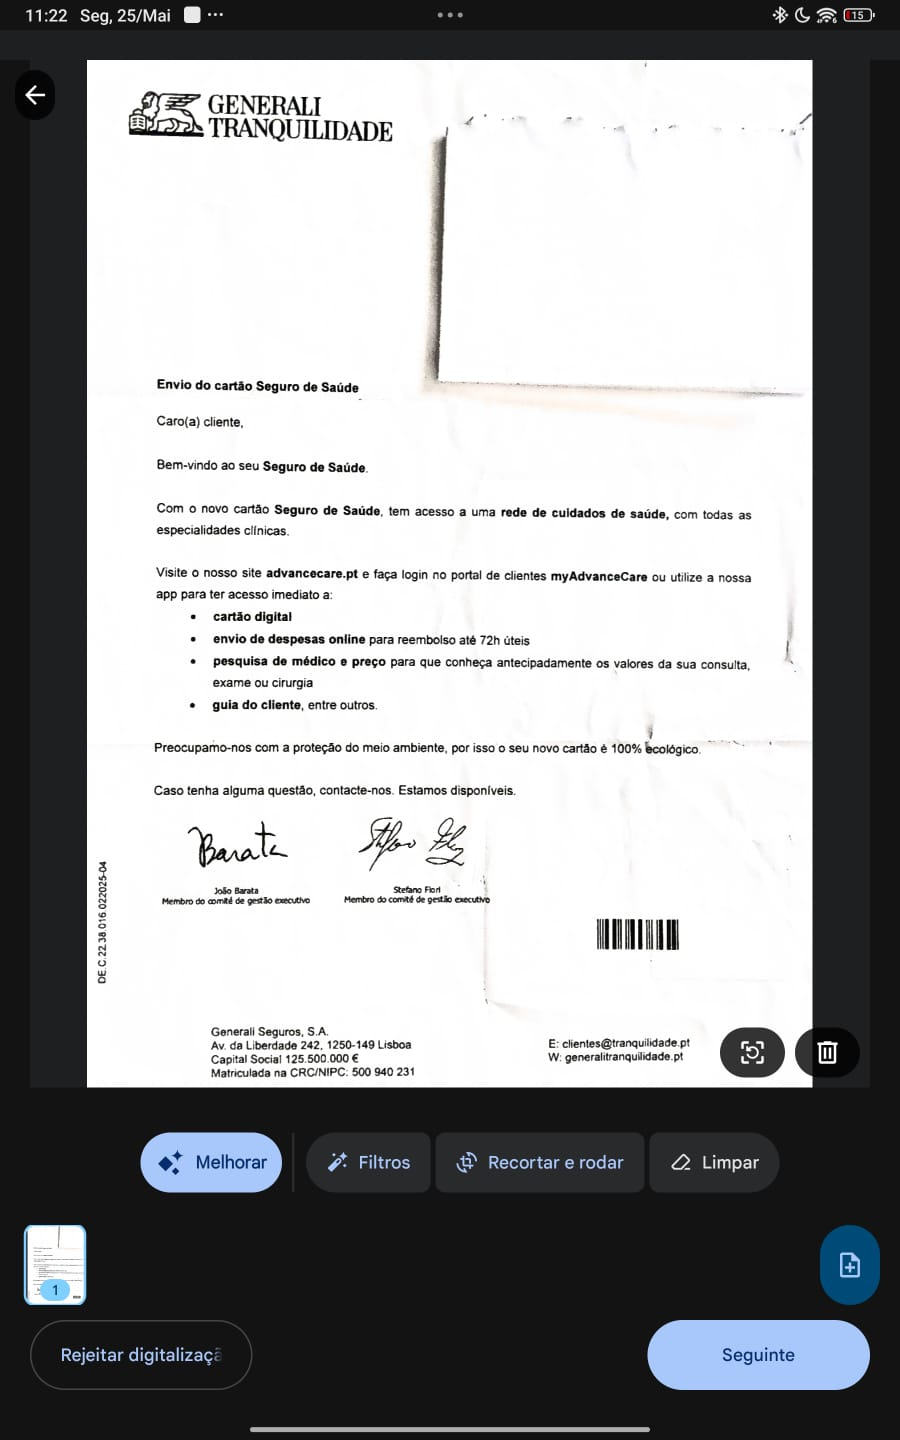
\includegraphics[width=\textwidth]{images/screenshots/scan_screen_2.jpeg}}
        \caption{Pré-visualização da Digitalização}
    \end{subfigure}
    \caption{Adição de documentos por \textit{upload} e digitalização.}
    \label{fig:manual-upload}
\end{figure}

\clearpage
\section{Processamento pela IA}

Após o \textit{upload}, o documento é processado automaticamente pela IA. O ecrã da esquerda da Figura~\ref{fig:manual-processing} mostra o indicador de progresso com as três fases do processamento. Quando concluído com sucesso, é apresentado o ecrã da direita com a mensagem ``Pronto a usar!'', permitindo ao utilizador navegar para o documento ou fazer um novo \textit{upload}.

\begin{figure}[H]
    \centering
    \begin{subfigure}[b]{0.28\textwidth}
        \centering
        \fbox{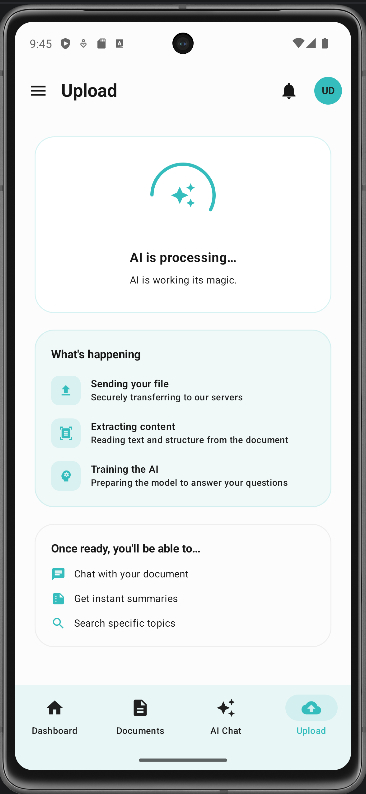
\includegraphics[width=\textwidth]{images/screenshots/upload_doc_moment_screen.png}}
        \caption{A Processar}
    \end{subfigure}
    \hspace{0.03\textwidth}
    \begin{subfigure}[b]{0.28\textwidth}
        \centering
        \fbox{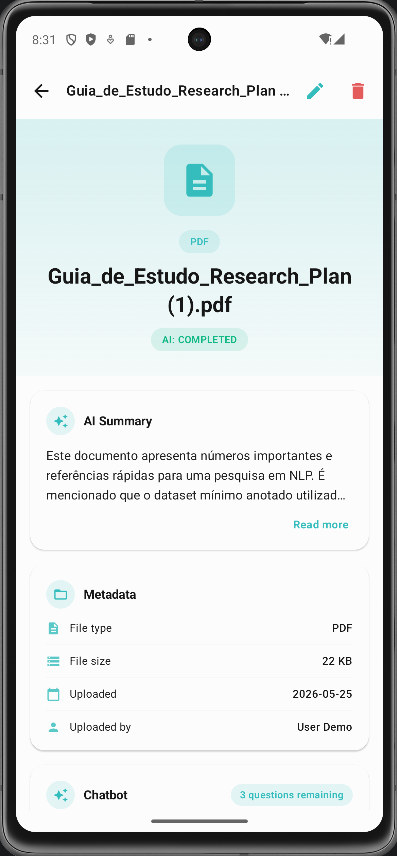
\includegraphics[width=\textwidth]{images/screenshots/completed_upload.png}}
        \caption{Processamento Concluído}
    \end{subfigure}
    \caption{Estados de processamento da IA após \textit{upload}.}
    \label{fig:manual-processing}
\end{figure}

\clearpage
\section{Chat Global}

O \textit{Chat} Global, acessível pelo separador de conversa na barra de navegação, permite ao utilizador fazer perguntas sobre todos os documentos da organização em simultâneo. O utilizador escreve a questão e toca em enviar; a IA pesquisa os documentos mais relevantes e apresenta a resposta com as fontes utilizadas e a percentagem de relevância de cada uma, como mostra o ecrã da direita da Figura~\ref{fig:manual-global-chat}. O número de perguntas disponíveis é apresentado no topo do ecrã.

\begin{figure}[H]
    \centering
    \begin{subfigure}[b]{0.28\textwidth}
        \centering
        \fbox{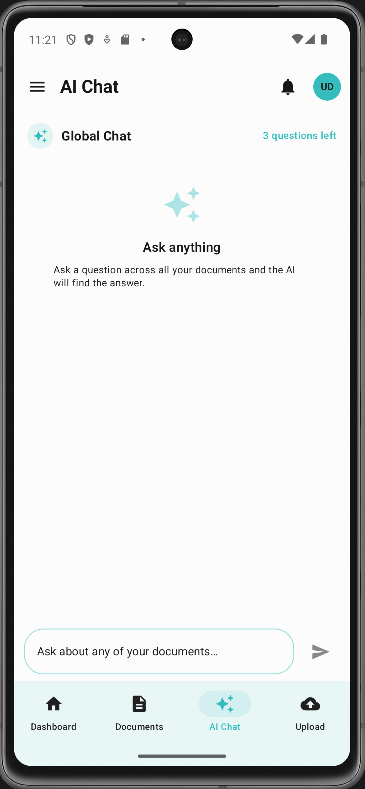
\includegraphics[width=\textwidth]{images/screenshots/global_chat.png}}
        \caption{\textit{Chat} Global}
    \end{subfigure}
    \hspace{0.03\textwidth}
    \begin{subfigure}[b]{0.28\textwidth}
        \centering
        \fbox{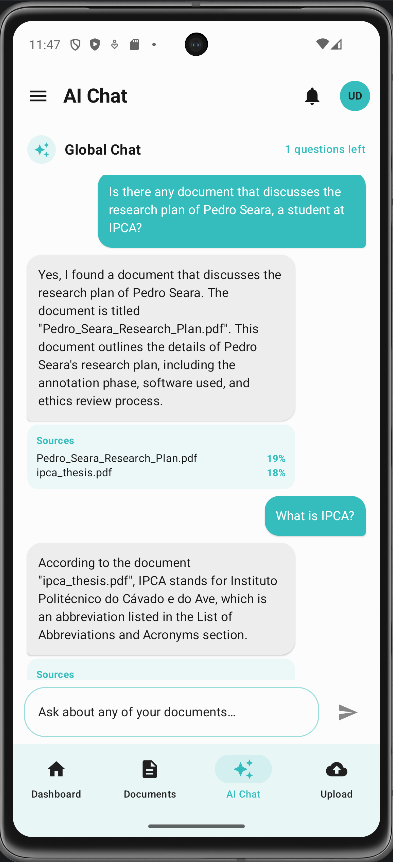
\includegraphics[width=\textwidth]{images/screenshots/global_chatbot_responses.png}}
        \caption{Fontes da Resposta}
    \end{subfigure}
    \caption{\textit{Chat} Global com RAG e indicação das fontes utilizadas.}
    \label{fig:manual-global-chat}
\end{figure}

\clearpage
\section{Notificações}

A aplicação recebe notificações \textit{push} no dispositivo mesmo com a app fechada. Ao tocar numa notificação recebida, a aplicação abre automaticamente no ecrã correspondente.

Os eventos que geram notificações são:

\begin{itemize}
    \item \textbf{Documento carregado} — confirmação de que o ficheiro foi recebido com sucesso;
    \item \textbf{Processamento IA concluído} — a análise automática do documento está disponível;
    \item \textbf{Convite de organização} — o utilizador foi convidado para uma organização;
    \item \textbf{Conta criada} — confirmação de criação de conta;
    \item \textbf{Formulário de contacto enviado} — confirmação de envio da mensagem de suporte.
\end{itemize}

Ao tocar no ícone de notificações na barra de navegação, o utilizador acede ao histórico, organizado nos separadores ``Não lidas'' e ``Todas'', como mostra a Figura~\ref{fig:manual-notifications}. As notificações não lidas são assinaladas visualmente. Tocar numa notificação individual marca-a como lida. O utilizador pode também marcar todas como lidas, limpar o histórico ou eliminar notificações individualmente.

\begin{figure}[H]
    \centering
    \begin{subfigure}[b]{0.28\textwidth}
        \centering
        \fbox{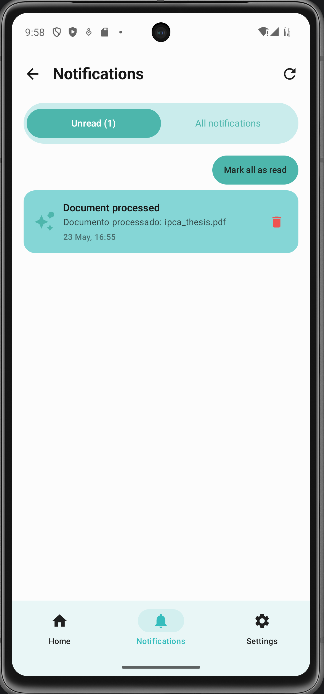
\includegraphics[width=\textwidth]{images/screenshots/unread_notifications_screen.png}}
        \caption{Não Lidas}
    \end{subfigure}
    \hspace{0.03\textwidth}
    \begin{subfigure}[b]{0.28\textwidth}
        \centering
        \fbox{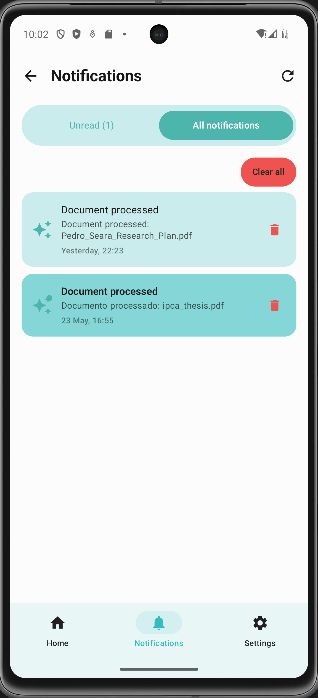
\includegraphics[width=\textwidth]{images/screenshots/all_notifications_screen.png}}
        \caption{Todas}
    \end{subfigure}
    \caption{Ecrã de notificações.}
    \label{fig:manual-notifications}
\end{figure}

\clearpage
\section{Perfil e Definições de Conta}

Ao aceder ao perfil através do menu lateral, o utilizador vê as suas informações de conta no ecrã da esquerda da Figura~\ref{fig:manual-profile}. Ao tocar em ``Editar Perfil'', pode alterar o nome, apelido e nome de utilizador e guardar as alterações. Para alterar a palavra-passe, seleciona ``Alterar Palavra-Passe'' nas definições, introduz a palavra-passe atual e a nova, e confirma, como mostra o ecrã da direita.

\begin{figure}[H]
    \centering
    \begin{subfigure}[b]{0.28\textwidth}
        \centering
        \fbox{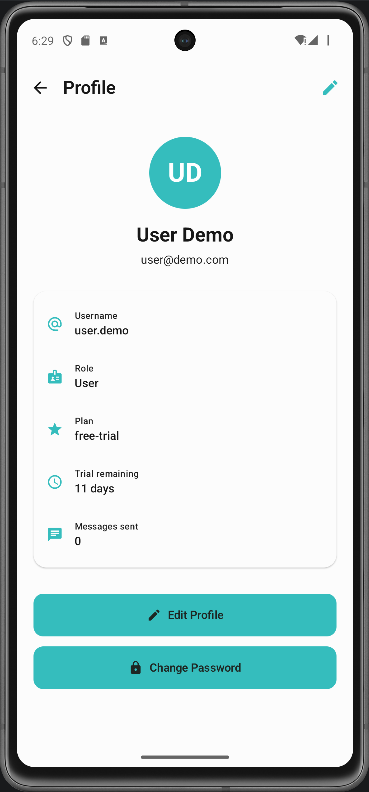
\includegraphics[width=\textwidth]{images/screenshots/profile_screen.png}}
        \caption{Perfil}
    \end{subfigure}
    \hspace{0.03\textwidth}
    \begin{subfigure}[b]{0.28\textwidth}
        \centering
        \fbox{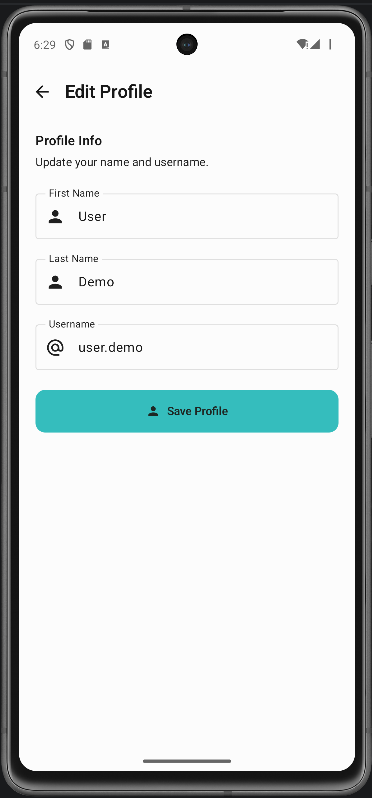
\includegraphics[width=\textwidth]{images/screenshots/edit_profile_screen.png}}
        \caption{Editar Perfil}
    \end{subfigure}
    \hspace{0.03\textwidth}
    \begin{subfigure}[b]{0.28\textwidth}
        \centering
        \fbox{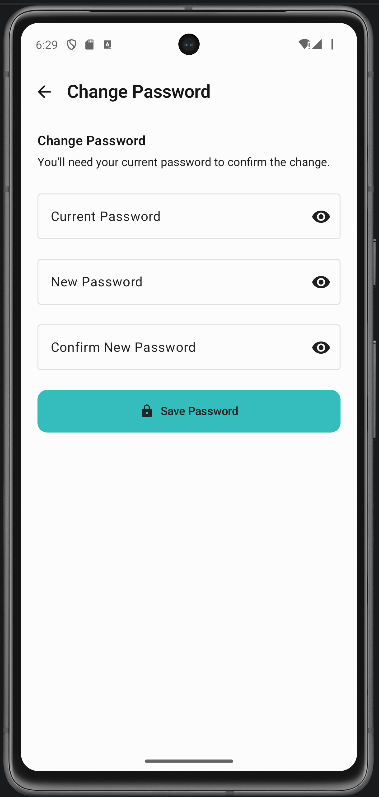
\includegraphics[width=\textwidth]{images/screenshots/change_password_screen.png}}
        \caption{Alterar Palavra-Passe}
    \end{subfigure}
    \caption{Ecrãs de perfil, edição e alteração de palavra-passe.}
    \label{fig:manual-profile}
\end{figure}

\clearpage
\section{Menu Lateral, Tema e Idioma}

O menu lateral é aberto tocando no ícone $\equiv$ no canto superior esquerdo, dando acesso rápido ao perfil, notificações, definições, ajuda e encerramento de sessão. Nas definições, o utilizador pode escolher o tema da aplicação entre \textbf{Claro}, \textbf{Escuro} ou \textbf{Sistema}, e o idioma entre \textbf{Português} e \textbf{Inglês}, como mostram os ecrãs da Figura~\ref{fig:manual-drawer}. As preferências são aplicadas de imediato.

\begin{figure}[H]
    \centering
    \begin{subfigure}[b]{0.28\textwidth}
        \centering
        \fbox{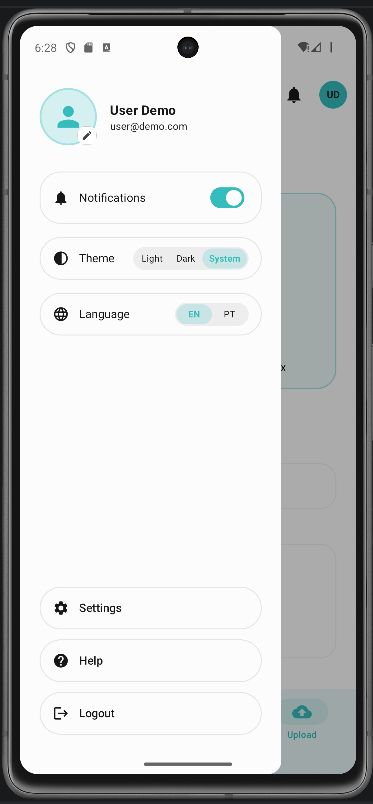
\includegraphics[width=\textwidth]{images/screenshots/side_bar_screen.png}}
        \caption{Menu Lateral}
    \end{subfigure}
    \hspace{0.03\textwidth}
    \begin{subfigure}[b]{0.28\textwidth}
        \centering
        \fbox{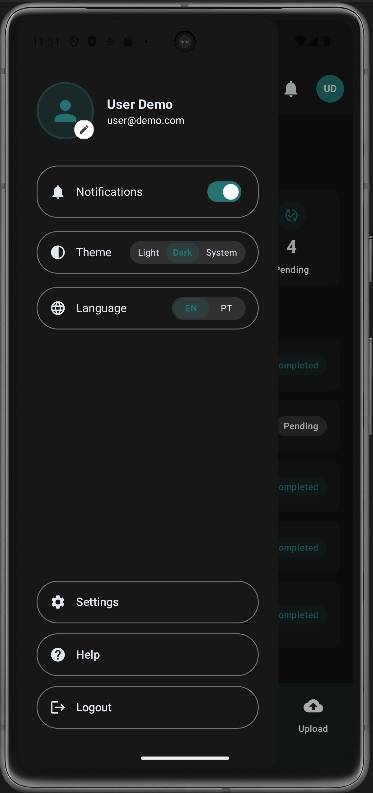
\includegraphics[width=\textwidth]{images/screenshots/dark_mode.png}}
        \caption{Tema Escuro}
    \end{subfigure}
    \caption{Menu lateral com seleção de tema e idioma.}
    \label{fig:manual-drawer}
\end{figure}

\clearpage
\section{Ajuda e Contactos}

Ao tocar em ``Ajuda'' no menu lateral, o utilizador é direcionado para o Centro de Ajuda, apresentado no ecrã da esquerda da Figura~\ref{fig:manual-help}, onde pode consultar as perguntas frequentes sobre a aplicação. Ao tocar em ``Contactar-nos'', é aberto o ecrã da direita, que apresenta simultaneamente o formulário de contacto e um mapa Google Maps com o marcador da localização da equipa. O utilizador preenche o nome, \textit{email}, assunto e mensagem e toca em ``Enviar''.

\begin{figure}[H]
    \centering
    \begin{subfigure}[b]{0.28\textwidth}
        \centering
        \fbox{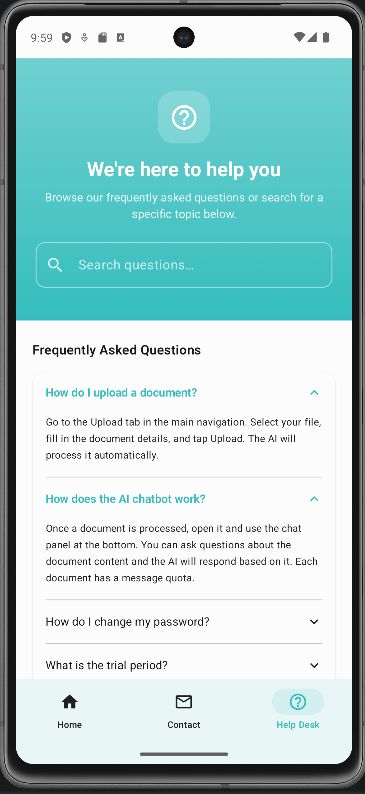
\includegraphics[width=\textwidth]{images/screenshots/help_faq_screen.png}}
        \caption{Centro de Ajuda}
    \end{subfigure}
    \hspace{0.03\textwidth}
    \begin{subfigure}[b]{0.28\textwidth}
        \centering
        \fbox{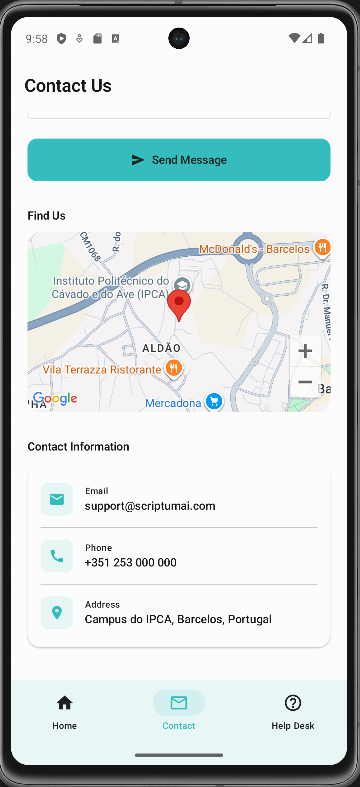
\includegraphics[width=\textwidth]{images/screenshots/contact_us_map_screen.png}}
        \caption{Contactar-nos}
    \end{subfigure}
    \caption{Centro de ajuda e ecrã de contacto com mapa de localização.}
    \label{fig:manual-help}
\end{figure}

\clearpage
\section{Modo Sem Ligação}

Quando o dispositivo não tem acesso à internet, a aplicação continua a funcionar em modo de leitura, apresentando os documentos guardados em cache local. O utilizador pode consultar o conteúdo dos documentos previamente acedidos sem necessidade de ligação. As funcionalidades que requerem servidor — como o \textit{upload}, a análise por IA e o \textit{chat} — ficam indisponíveis até a ligação ser restabelecida.
